\section{Crittografia a chiave Pubblica (asimmetrica)}

La crittografia asimmetrica, conosciuta anche come crittografia a coppia di chiavi,
crittografia a
chiave pubblica/privata o anche solo crittografia a chiave pubblica, è un tipo
di crittografia dove ad
ogni attore coinvolto nella comunicazione è associata una coppia di chiavi:

\begin{itemize}
    \item La chiave pubblica, che deve essere distribuita;
    \item La chiave privata, appunto personale e segreta;
\end{itemize}

Fra due interlocutori, non vi è dunque la necessità di scambiarsi le chiavi.
Se con una delle due
chiavi si cifra (codifica) un messaggio, allora quest'ultimo sarà decifrato solo
con l'altra.

\begin{figure}[H]
    \centering
    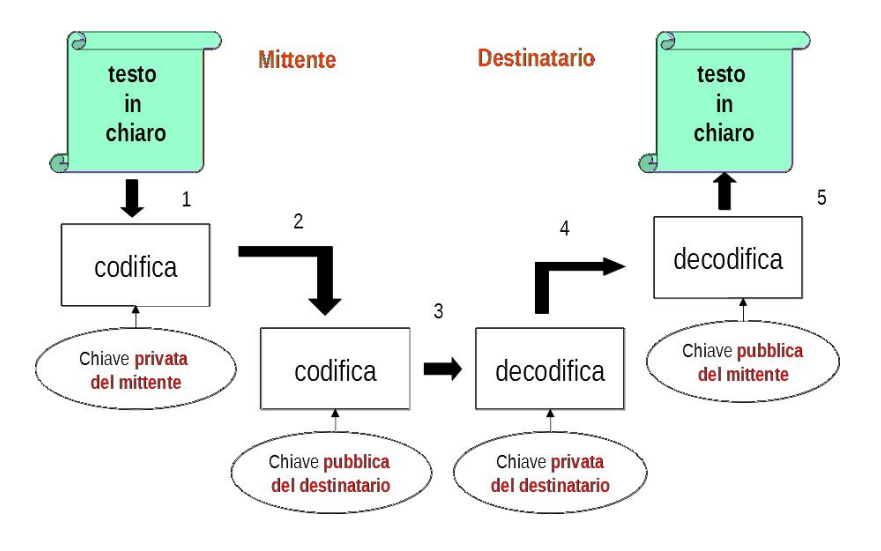
\includegraphics[width=\textwidth, keepaspectratio]{capitoli/crittografia/imgs/pubblica.png}
    \caption{Esempio del funzionamento della Crittografia Asimmetrica.}
\end{figure}

Gli attacchi a sistemi di crittografici sono detti attacchi
di \textbf{Crittoanalisi} e
come obbiettivo hanno quello di provare a dedurre la chiave che gli
permetterebbe di decriptare il testo.
I principali attacchi crittografici si basano sulle seguenti caratteristiche:

\begin{itemize}
    \item \textbf{CypherText only}: è noto solo il testo codificato;
    \item \textbf{Known plaintext}: il messaggio è cifrato ma il testo in chiaro è noto;
    \item \textbf{Chosen plaintext}: il testo in chiaro viene scelto in quale modo (per es. tutti 0, tutti 1, ecc);
    \item \textbf{Brute-force}: forza bruta, tentativi di attacco alla chiave finché non si trova quella giusta;
\end{itemize}

\paragraph{Crittografia Perfetta: } la crittografai si di dice Perfetta quando
nessun
testo codificato rilascia informazione alcuna né
sulla chiave usata per la codifica, né sul testo in chiaro,
il quale può essere recuperato se e solo se
la chiave è disponibile.
Si tratta di una situazione ideale, in quanto ogni tipo di crittoanalisi sarebbe
reso inutile e la
probabilità di ricavare informazioni supplementari da un testo codificato
sarebbe piuttosto nulla.
Purtroppo però, la crittografia in pratica non è quasi mai perfetta.
